\vspace{0.5cm}
Al leer el archivo con las siguientes líneas de código
\begin{lstlisting}
sscanf(content, "%s %f %f %f %f %f %f",head, &rest, &rest, &cumulative, &count,&rest, &rest);

        if(strcmp(head, "M") == 0 ){

            printf("%d \t %f \n",i,count);

            H1->SetBinContent(i,count);
            i++;
        }
\end{lstlisting}
En donde se hace la distinción de las líneas que inician con "M". Con esto se genera un histograma que claramente se asemeja a una distribución de Poisson, al menos al inicio.

\begin{figure}[H]
	\centering
	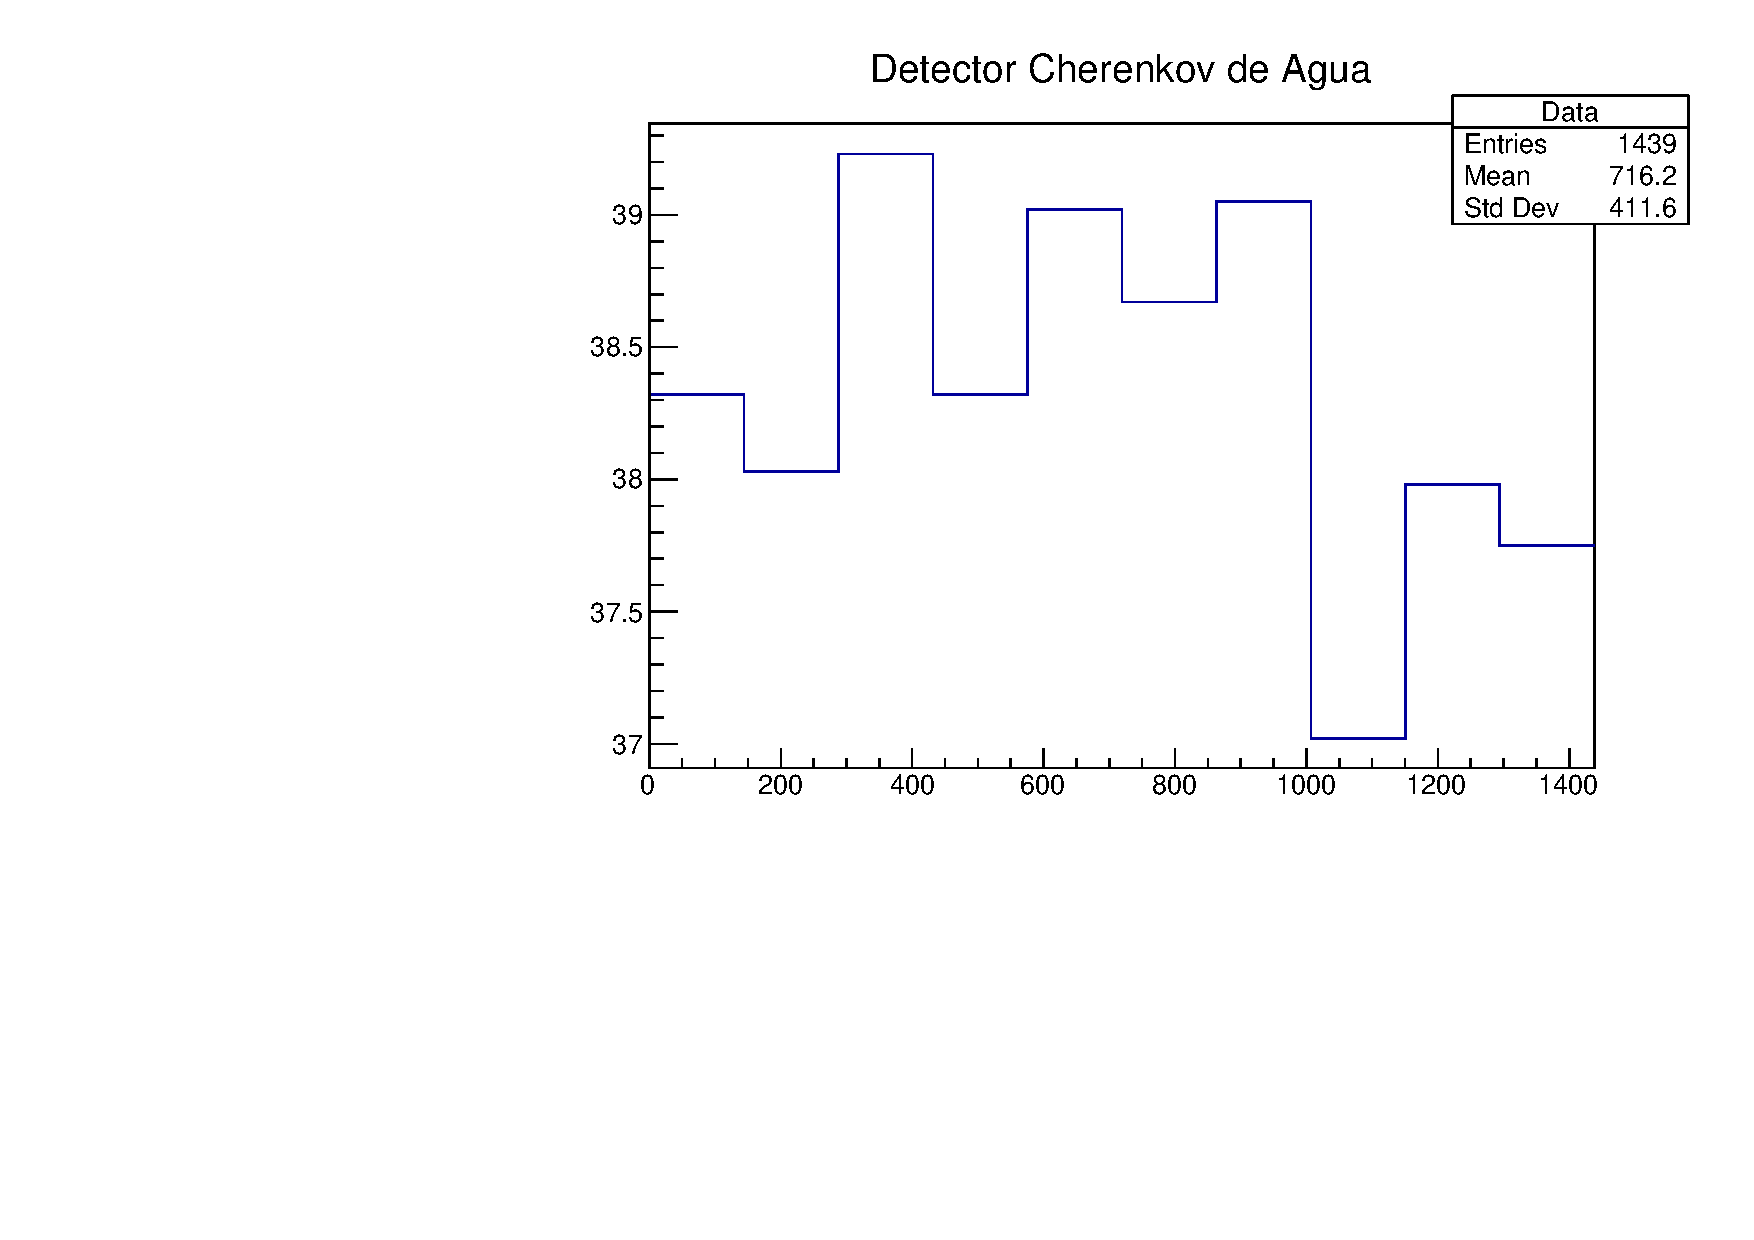
\includegraphics[scale=0.5]{histograma.pdf}
	\caption{Histograma}
	\label{hist}
\end{figure}